%%% Time-stamp: <2015-04-15 00:55:14 sunthar>

%%% $Log:$

%\documentclass[11pt,a4paper,openright]{report}
\documentclass[seminar,twoside]{iitbreport}


%% Selectively comment out sections that you want to be left out but
%% maintaining the page numbers and other \ref
\includeonly{%
  chapter1/introduction,
  chapter2/background,
}  
%expt/experimental,
%rnd/results,


%%% Some commonly used packages (make sure your LaTeX installation
%%% contains these packages, if not ask your senior to help installing
%%% the packages)


\usepackage{booktabs}
\usepackage{url}
\graphicspath{{expt/}}


%%% Macro definitions for Commonly used symbols
\newcommand{\etas}{\ensuremath{\eta_{\mathrm{s}}}}
\newcommand{\Rey}{\ensuremath{\mathrm{Re}}}
\newcommand{\avg}[1]{\ensuremath{\overline{#1}}}
\newcommand{\tenpow}[1]{\ensuremath{\times 10^{#1}}}

\newcommand{\pder}[2]{\ensuremath{\frac{\partial#1}{\partial#2}}}


% Referencing macros
\newcommand{\Eqref}[1]{Equation~\eqref{#1}}
\newcommand{\Tabref}[1]{Table~\ref{#1}}
\newcommand{\Figref}[1]{Figure~\ref{#1}}
\newcommand{\Appref}[1]{Appendix~\ref{#1}}

%Command for including image source
\newcommand*{\captionsource}[3]{%
  \caption[{#1}]{%
	#2%
    \\\hspace{\linewidth}%
    \textbf{Source:} #3%
	}%
}


\begin{document}
\title{Study of Virtualization \& Management of Memory in Virtualized Systems}
\author{Aby Sam Ross\\143050093}
%\date{\today}
\degree{Master of Technology}
\dept{Computer Science \& Engineering}
\monthyear{April 2015}

%\makecoverpage
\maketitle

\begin{abstract}
Memory like other computing resources can be considered a scarce enough commodity. Multiplexing
and management of this memory among various stakeholders in native computing environments has been
well taken care of. But when it comes to virtualized environments it adds another layer of
abstraction. This calls for new techniques, for partitioning and arbitrating memory among
different VMs, that doesn't change the OS's perspective of the scheme of things and requires
minimal changes. While the techniques for partitioning memory among different VMs in a virtualized
setting has almost got standardized, there are still differing views and different approaches to
managing memory. The new layer of abstraction introduced by virtualization adds considerable
complexity in estimating the needs and utilization of memory. One cannot retrofit one strategy
suitable for a particular setting to another and expect to get a clear picture of memory related
parameters. This seminar is to understand different techniques of memory virtualization and to gain some insight into some of the existing management strategies.
 
\end{abstract}

\pagenumbering{roman}
\tableofcontents

%\listoftables
\listoffigures

%\cleardoublepage
\setcounter{page}{1}
\pagenumbering{arabic}


\chapter{Introduction}

\section{Overview of Virtualization}
Hardware resource abstraction and management have always been a major aim and challenge in
electronic systems. With the advent of computers these tasks fell upon a huge piece of software
called the Operating System. It became the responsibility of the OS to multiplex the resources
among the different processes running in a system. An obvious illustration is that of CPU
multiplexing, where the CPU is scheduled in time slices among various processes according to
priority. The physical memory in a system as well is a resource. Memory also needs to be
abstracted and suitable interfaces are to be provided for easy and efficient use. Traditionally
this has been achieved through the concept of virtual memory coupled with paging or segmentation.
\\
With advancements in technology the capabilities of physical resources increased and cost
decreased. Processors and memory became faster, smaller chips with more capacity became available.
But these advancements didn't percolate naturally into better utilization of these resources.
Often these resources were underutilized. In order to get better utility from these resources
various options of sharing these resources at a larger granularity was explored. Thus came into
existence the concept of virtualization.\\
Virtualization increases the granularity of abstraction from individual resources to abstracting
the entire set of hardware as a single unit or in other words virtualization abstracts the entire
computer system. With this we could have more than one machine running on top of the existing
computing hardware. These machines came to be called \textit{Virtual Machines} or VM. In other
words with the increase in granularity of abstraction the unit of allocation to the abstraction
increased from a process to an entire OS.\\
The ringmaster who runs the show in a Virtual Machine is still the humongous piece of code called
the OS. But traditionally OSes were designed to have ownership and control of the underlying
hardware. Virtualization now created a separation between the hardware and the OS.They were now
relegated to the status of a \textit{guest OS}. A single OS was no longer the sole owner and
controller of the resources. The entire hardware had to be abstracted, interfaced and multiplexed
among different OSes manning different VMs analogous to the way in which an OS enabled
multiplexing of resources among different processes in a native system. This role was now taken up
by a new, but no less hideous, software layer called the \textit{Virtual Machine Monitor} (VMM) or
the \textit{Hypervisor}. That is now we have the hypervisor sitting on top of the hardware 
directly and above it we have different VMs.\\
The introduction of a new orchestrator, the Hypervisor, and relegation of a guest OS to a lesser
privilege brought about new challenges. The guest OS in a VM had no longer complete control of the
underlying resources to arbitrate efficiently among the processes running in it. But to the
process local to a VM the guest OS was still the ringmaster who ran the show. Hence it became of
paramount importance that the introduction of a software layer, the hypervisor, between the guest
OS and the resources didn't break the equivalence view  i.e. a process running in a VM should see
no or little difference in running on a native vs. virtualized system. At the same time we also
had to ensure that every VM stayed within its allocated bounds and guest OS operations had enough
efficiency. These requirements of hypervisor design are formally stated in Popek and Goldberg
\citep{Popek1974}.The hypervisor can choose from among the various strategies like instruction
interpretation, trap \& emulate, binary translation, para-virtualization, hardware assisted
virtualization to provide the aforementioned requirements.\\
Once such a hypervisor is available efficient resource utilization and management comes next in
order to meet the original design principles of virtualization. Memory like other
resources will also be apportioned to the different VMs. But it is not necessary that all  of the
memory allocated to a VM will be in 100\% use all the time. This gives us an opportunity to
reallocate this unused memory to other VMs in need. But its sharing and management is not as
simple as that of a flexible resource like CPU and nor are the effects of differences in the
amounts of memory available that easily visible \citep{Mortar2014}. The objective of this seminar is to get an understanding of the intricacies involved in this. 

\section{Scope of the Seminar}
The objective of this seminar is not to delve deep into the implementation of virtualization as a whole but rather to concentrate on understanding how memory virtualization is achieved,  
\begin{itemize}
\item Unnumbered and Numbered Lists
\item Equations
\item Defining short macros for frequently used symbols
\item Bibliography
\item Figures
\item Tables
\end{itemize}

The normal procedure for compiling a \LaTeX\ document that contains
bibliographic entries is to follow the following steps
\begin{enumerate}
\item \verb|pdflatex mainrep|
\item \verb|bibtex mainrep|
\item \verb|pdflatex mainrep|
\item \verb|pdflatex mainrep|
\end{enumerate}
In the above example \verb|mainrep| is the main \LaTeX\ file.




This is the first chapter, which resides in a directory (folder)
intro. Each chapter can contain \verb|section|, \verb|subsection|
and so on.




Equations should be set in a separate mode.  For details on getting
various types of aligned equations, consult the \AmS-\LaTeX\
documentation \verb|amsldoc.pdf|. Simple equations are set as
\begin{equation}
\label{eq:sinx}
\int \mathrm{d}x \; \cos x =  \sin x
\end{equation}
Equation~\eqref{eq:sinx} is the integral of the cosine
function. Mathematical symbols must always be put inside \verb|$$|,
when they appear outside a math environment (such as \verb|equation|,
\verb|align|, \verb|gather|, etc).  The symbol ``ex'' must be written as
$x$ and not as x.  

Another commonly used construct for equations is the \verb|align|
environment to align several equations along a vertical line. It is
usually the $=$ sign across which the alignment is done.  The
point of alignment for each equation is specified using the ampersand symbol 
\begin{align}
a &= b  \\
a + e + f + g & = m + n + z \\
x + 2 & = x^{3} + 3 x^{2} + 2 x + 5
\end{align}

\subsection{Commonly used Symbols}
For mathematical symbols it is very convenient to define frequently
used symbols as a short macro. For example if you are to be using the
symbol $\eta_{\mathrm{s}}$ frequently it is convenient to define it in
as:\\
\verb|\newcommand{\etas}{\ensuremath{\eta_{\mathrm{s}}}}| \\
in the preamble and to simply refer it to in the text as \etas\ or in
a mathematical equation as $\etas = \eta \, ( 1 + \phi)$.

%%% Local Variables: 
%%% mode: latex
%%% TeX-master: "../mainrep"
%%% End: 

\chapter{Background}

\section{Memory Management in Native Systems} \label{native}
Memory management in non-virtualized native multiprogramming system is achieved using Virtual
Memory. In multiprogrammed systems several programs are resident in memory at the same time.
The memory management policy in such a system deals with protecting the memory of one program from 
another, loading a program into available space in main memory, (de)allocating memory dynamically
from/to programs.\\
While programs are complied and linked with addresses starting at $0$ and CPU uses 
these addresses to access the binary, it isn't necessary (and is the not the case that) that a
program will get physical memory with the same addresses or it is not even guaranteed that there
will be enough space in the physical memory to load the entire binary of the program. Most of the
times only the immediately needed part of the program is loaded onto the available physical
memory, (the rest will be held in a backing store - often the hard disk) and they will share the
physical memory space along with parts of other programs. And the OS may choose to evict parts of
the program to the backing store when in need of memory as a part of its memory management policy.
Therefore the addresses generated by CPU needs to be translated into the corresponding physical
addresses. The address generated by CPU is called \textit{Virtual Address} or VA . Thus we need to
have a mechanism of \textit{Virtual Address (VA)} $\rightarrow$ \textit{Physical Address (PA)}
translation.\\
Hence the illusion that is given to a program that there is enough physical memory available to
store its entire binary combined with relocation of code having contiguous virtual addresses into
- not necessarily contiguous - available physical memory chunks are the central ideas of virtual
memory.\\
Virtual Memory can be implemented in more than one ways. Paging is one of them. The idea behind
paging is to divide the virtual address space and the physical memory into same sized units of
allocation called \textit{pages}. Hence the virtual address space is divided into \textit{virtual
pages} or simply \textit{pages} and physical memory into \textit{physical pages} or
\textit{frames} or \textit{physical/machine frames}. It is thus clear that not all pages of a
program will be present in the physical memory when the program is executing, the contiguous
virtual pages belonging to the same program needn't be allocated contiguous frames and it is
necessary to provide a way to map from the virtual pages to the associated machine frames.\\
This mapping should be there for each program and this mapping is called the \textit{page table}.
The organisation of page table is closely tied to the size of a page or a frame. Page size is
taken as \textit{power of 2} as this ensures that all binary representable addresses can be
utilized and address manipulation can be done without arithmetic operations. There should an be an
entry for all virtual page addresses of a program in its page table. This will result in a very
long (large) page table and all the page tables of all programs that are currently resident in
memory will consume considerable amount of physical memory. So instead of storing such a single
large page table per program in memory we break the page tables into different levels to have a
tree like structure. Thus following the design principles of virtual memory it is not necessary
that even all the levels of the page table will be resident in memory all the time.\\
Often the entries in each level are grouped into different sets. And each entry will contain a
physical address and some flag bits. The flag bits store permissions and other info about the this
entry and the physical address in the entry points to a set of entries in the next level. These
sets of entries in each level are often limited to single physical frame. Thus the physical
address in a page table entry points to a physical frame in the next level. There is an exception
for the last level of the page table. An entry in the last level contains the physical address of
the actual virtual page that we were looking for and the flag bits of the entry include
information like whether the physical page it points to is present or not. The physical address of
the root of the page table (i.e. the physical address of the base of the outermost level of page
table) is stored in a hardware register.\\
The translation of virtual address to physical address happens in the following manner:\\
The base address of the program's page table is obtained from the hardware register storing it. To
this base address we add that part of the virtual address that corresponds to the outermost level. 
Thus we get the corresponding entry in the outer most level which points to the base address of
the corresponding set of entries of the next level (i.e. a physical page of the next level) . Now
to get to the corresponding entry within that physical page we add the part of virtual address for
the next level to the physical page address we obtained from the outermost level. This process is
continued till we get to a last level entry from which we get the physical frame address 
corresponding to the virtual address. And to go to the exact physical address location
corresponding to the virtual address location add the last part of the virtual that doesn't
correspond to any page table level i.e. the offset part to the physical frame address.\\    
Hence it is clear from the above discussion that the parts of the virtual address that correspond
to each level of page table give us an offset within that level and last part of the virtual
address that doesn't correspond to any page table level gives us the offset within the actual
frame that holds this virtual address. Illustration in figure \ref{fig:pagetable}.\\
For a virtual address generated by the CPU the translation to physical address i.e. traversing the
levels of page table happens in hardware. If the corresponding physical page is present in the
translated location it is a \textit{hit} else it is a \textit{fault}. Page faults are to be
resolved by moving in the corresponding missing page from the backing store. Certain architectures
like x86 choose to cache recently accessed virtual addresses and their mappings in a small cache
often called the \textit{translational look ahead buffer} or TLB, this is for faster translations
the next the same address is accessed. This also brings about the need for coherence between the
entries in the TLB and the page table. The hardware that does all this is called the
\textit{memory management unit} or MMU.\\
Linux OS on x86 (i.e. 32 bit) architecture has 3 levels of the page table. While for x86\_64 (i.e.
64bit) it has 4. They are called \textit{page global directory} or PGD, \textit{page upper
directory} or PUD, \textit{page middle directory} or PMD and \textit{page table entry} or PTE. x86
won't have the PMD. The \textit{CR3} register holds the base address of the PGD.\\

\begin{figure}[tbp]
  \begin{center}
    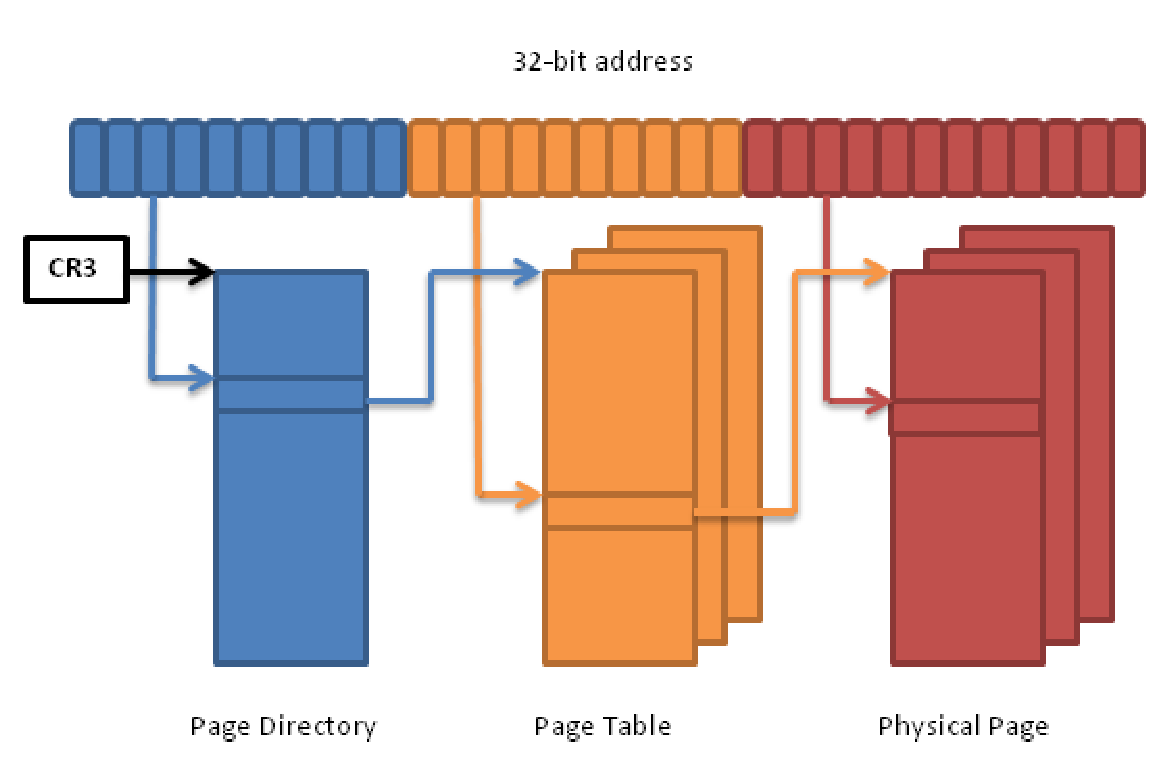
\includegraphics[width=0.7\textwidth]{images/pagetable}
        	%\caption[Page Table Illustration]{Illustration of \textit{VA} $\rightarrow$ \textit{PA} address translation.}
        	\captionsource{Page Table Illustration}{Illustration of \textit{VA} $\rightarrow$ \textit{PA} address translation.}{\url{corensic.files.wordpress.com/2011/11/virtualmemory.png}}  
    \label{fig:pagetable}
     \end{center}
\end{figure}

\section{Challenges to Virtualizing Memory} \label{challenges}
When we introduce virtualization the physical memory of the system is to be shared among different
VMs. In addition to that there should be ways to dynamically (re)allocate memory among VMs
analogous to the way in which memory is managed among programs in a native system as discussed in
the previous sections. Hence the basic idea of memory virtualization is similar to virtual memory
in native systems. Here on top of the virtual memory abstraction that happens inside a VM we are
introducing another layer of virtual memory sort of abstraction. If we want minimal changes to a
stock guest OS or if the guest OS is unaware of the underlying hypervisor then the guest OS's
perceived view of physical memory should be kept intact by allowing it to maintain the mapping of
virtual addresses to what the guest OS perceives as its physical memory. While in reality what the
guest OS perceives as physical memory is not the real machine memory and neither is it given
unrestricted direct access to the entire real machine memory. This was done to ensure that guest
OSs stay within their bounds and VM isolation was guaranteed. Moreover guest OSs no longer managed
the resources on their own.\\
This was achieved by virtualizing the MMU or in other words by introducing MMU functionalities in
the hypervisor level that backed the the guest OS memory management operations, trying as far as
possible not to break the guest OS's view of the affairs, and that did effective multiplexing of
actual machine memory among the different VMs.\\
Implementing this is not as easy as said. The first challenge lies in deciding how to divide or
partition machine memory among different VMs. Dictating the techniques of access poses another.
Finally the dynamic management aspect comes in.\\
Every VM can be allocated simple, static, contiguous, disjoint fixed partitions or more of a
dynamic allocation scheme similar to demand paging discussed in previous section can be adopted.
The former has obvious drawbacks of memory wastage if the allocated memory is underutilized,
incapability to support a VM requiring more memory than the static allocation etc. All this will
affect the number of VMs that can be hosted on a machine. In addition it cannot support other
virtualization techniques like migration. 
The latter ensures better utilization of memory, enables memory over-commitment among VMs, similar
to the one provided to different processes by normal virtual memory, but introduces considerable
complexity in implementation. One reason for this complexity is the varying levels of dynamism in
memory demands among different VMs which requires the VMM to detect and react quickly to these
demands by adapting its policies for each VM. Another cause of this complexity is multiple memory
resource control entities taking decisions independently; one the guest OS and other the VMM. This
can often result in conflicting decisions being made that increases the memory management
overhead.\\
Since the guest OS employs virtual memory, access to the MMU is often needed. But we also know the
actual MMU functionalities that manages the machine memory lies in the hyervisor. Thus hypervisor
needs to define ways for the guest OS to access these functionalities without breaking VM
isolation.\\
The challenges of implementing memory management at the hypervisor comes next. First, a VMM needs
to accurately determine memory resource usage statistics of individual VM to take any management
policy related decision. Second, policy decisions taken at the VMM level can clash with the
decisions taken within a guest OS. A good example of this the is \textit{double paging} explained
in \citet{waldspurger2002memory}. Third, it is difficult to define a one-copy-fits-all management
strategy for the various types of guest OSs and applications running in different VMs. For e.g. an
application like DB which manages its own memory will be affected badly by a VMM memory management
strategy that transparently reallocates memory assigned to it because for efficient working these
applications need a current, consistent view of the memory allocated to it
\citep{salomie2013application}.\\ 
We now try to look into the existing solutions and implementations of various aspects of memory
virtualization that address many of these issues. 

%\include{expt/experimental}
%\include{rnd/results}

\bibliography{mainrep}


\end{document}




%%% Local Variables: 
%%% mode: latex
%%% TeX-master: t
%%% End: 
